\documentclass{sigchi}

% Use this command to override the default ACM copyright statement (e.g. for preprints). 
% Consult the conference website for the camera-ready copyright statement.
\toappear{
Second draft
% Submitted for review.
}

% Arabic page numbers for submission. 
% Remove this line to eliminate page numbers for the camera ready copy
\pagenumbering{arabic}


% Load basic packages
\usepackage{balance}  % to better equalize the last page
\usepackage{graphics} % for EPS, load graphicx instead
%%\usepackage{graphicx}
\usepackage{times}    % comment if you want LaTeX's default font
\usepackage{url}      % llt: nicely formatted URLs

% llt: Define a global style for URLs, rather that the default one
\makeatletter
\def\url@leostyle{%
  \@ifundefined{selectfont}{\def\UrlFont{\sf}}{\def\UrlFont{\small\bf\ttfamily}}}
\makeatother
\urlstyle{leo}


% To make various LaTeX processors do the right thing with page size.
\def\pprw{8.5in}
\def\pprh{11in}
\special{papersize=\pprw,\pprh}
\setlength{\paperwidth}{\pprw}
\setlength{\paperheight}{\pprh}
\setlength{\pdfpagewidth}{\pprw}
\setlength{\pdfpageheight}{\pprh}

% Make sure hyperref comes last of your loaded packages, 
% to give it a fighting chance of not being over-written, 
% since its job is to redefine many LaTeX commands.
\usepackage[pdftex]{hyperref}
\hypersetup{
pdftitle={User Modeling in Exploratory Search},
pdfauthor={LaTeX},
pdfkeywords={SIGCHI, proceedings, archival format},
bookmarksnumbered,
pdfstartview={FitH},
colorlinks,
citecolor=black,
filecolor=black,
linkcolor=black,
urlcolor=black,
breaklinks=true,
}

\DeclareGraphicsExtensions{.pdf,.png,.jpg}

% create a shortcut to typeset table headings
\newcommand\tabhead[1]{\small\textbf{#1}}


% End of preamble. Here it comes the document.
\begin{document}

\title{User Modeling in Exploratory Search}

\def\tktl{Department of Computer Science\\University of Helsinki}
\def\tktladdr{P.O. Box 68 (Gustaf H\"allstr\"omin katu 2b)\\
FI-00014 UNIVERSITY OF HELSINKI\\
FINLAND}

\numberofauthors{2}
\author{
  \alignauthor Ilkka Kiistala\\
    \affaddr{\tktl}\\
    % \affaddr{\tktladdr}\\
    \email{ilkka.kiistala@helsinki.fi}
  \alignauthor Tuire Peurala\\
    \affaddr{\tktl}\\
    % \affaddr{\tktladdr}\\
    \email{tuire.peurala@helsinki.fi}
}

\maketitle

\begin{abstract}
Here we'll describe the content of our essay.
\end{abstract}

\keywords{
Exploratory Search; Information Retrieval; User Modeling.
}

\category{H.5.m.}{Information Interfaces and Presentation (e.g. HCI)}{Miscellaneous}


\terms{
Human Factors; Design; Measurement. 
}

\section{Introduction}
Context – who needs, what needs, why that is a problem in current situation 

We'll describe here the roles of further chapters.

\section{User modeling}
\label{sec:usermodeling}
Shortish explanation of user modeling key concepts. 
\cite{rich99}, \cite{fischer01}

To build a good system where machine and a human cooperate to perform a task it is important to take into account some significant characteristics of people \cite{rich99}. User model is built of these characteristics and traditionally it has been a model of a typical user \cite{rich99}. In reality often the users vary so much that a traditional user model is insufficient and there is a need for a user model of an individual.

\subsection{Sterotypes}
Modeling stereotypes. 
% HCI reference needed
\cite{dillon96}, \cite{pu02}
Traditional user models have been constructed by collecting data on an average user on various tasks and environments \cite{rich99}. An example of a sterotypical user model is Fitt's law that suggests that the speed on which the user operates the machine can be increased by increasing the size of targets the user must hit. The major weakness of these kind of models is that they assume that all the users constitute a homogenous set. In most cases for the majority of users the system is better adapted to them taht would be without any adaptation, but it isn't likely the best system that could be produced \cite{rich99}.

\subsection{How to Collect and Analyze User Information}
% Pazzani puhuu "user profileista"
\cite{pazzani97}, \cite{white10}

\subsection{Personalization}
Individualization of user models, Adaptive/Adaptable User Interfaces, intelligent user interfaces
\cite{bunt04}, \cite{findlater04}, \cite{brusi96}

\cite{van08}: "Personalized system's output or appearance differs for every user or user group in every context. The adapted output has the potential to be a great benefit for users; it is geared towards the user's preferences, behaviour or needs and it can make interaction easier and a lot more fruitful." The evaluation of a personalized system is problematic because it is unclear if the results gathered from a few individuals who all used system personalized for them can be generalized to entire population of users.

\cite{van08}: The writers are researchers at University of Twente, Netherlands. They took a look at scientific articles about “user-centered evaluation (UCE) studies of adaptive and adaptable systems”. The articles they reviewed are from 2007 and before. They reviewed 63 studies. Of the systems in the studies, 37 \% were adaptive, 27 \% adaptable and the rest, 36 \%, were both adaptive and adaptable. As a result of their literature review, they have modeled a process that can be used in evaluating a personalized system.
The model they present, “the iterative design process for a personalized system”, has four phases based on how ready the system is. Based on their findings in the studies they reviewed, they connect the most useful methods to use and most appropriate variables to investigate in each phase.
Overall, the article notes that “the current UCE practice of personalized systems was found to be sloppy at times”. They found that some of the questionnaires they reviewed were poorly designed and suggest that all the questionnaire data and log data as well should be made available so that a reader can judge the quality of the study. One reason they mention for low quality evaluations is that most evaluators of personalized systems are computer scientists and not specialized in evaluation.

\section {Exploratory search is a subtopic of information retrieval}

\subsection{Information retrieval}
There are many goals in information retrieval and exploratory search is one of them.
\cite{hearst02}, \cite{kuhlt91}

Information seekers often express a desire for a user interface that organizes search results into meaningful groups, in order to help make sense of the results and to help decide what to do next \cite{hearst06}. There two ways of grouping search results; clustering and hierarchical faceted categories. Clustering is grouping of items based on some similarity and is fully automated process. It is good for clarifying a vague query but the clustering algorithms aren't yet perfect and the clustering can be unpredicted \cite{hearst06}. Category system is a set of labels that are organized to mirror the domain. Hierarchical faceted categories are a set of hierarchical categories that each represent a different dimension. Categories are usually created manually but can be partly automated. 

\subsection{Exploratory Search}
Introduction to exploratory search.
\cite{march06}, \cite{white09}, \cite{tvaro11}

%% Palstan leveys tuntuu olevan n. 245pt

%\begin{figure}[p]
%\centering
%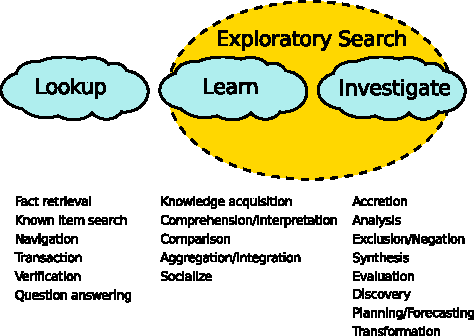
\includegraphics[bb=0 0 228 162]{clouds}
%\caption{Three clouds}
%\label{fig:clouds}
%\end{figure}

The user interface of an exploratory search system should be designed to fulfill the needs of most of its users. More information on what works and doesn't work can usually be collected from system evaluations.

However, evaluating exploratory search systems is difficult, because users have different starting positions. Their knowledge of the domain varies, they are interested in different aspects of the topic and they have previously encountered different information. \cite{kules08}

\section{User modeling in exploratory search}
Generally
\cite{oconnor10}, \cite{sugi04}, \cite{white07}, \cite{kules09}

\cite{kules09}:The writers had done a user experiment to find out what  the searchers are  looking at in a faceted search UI. The test participants were  university students and the system of interest was a library system. As a result  of the eyetracker test the writers found out that participants looked a lot at the facets and  47,4\% of the  eye movement  was between facets, breadcrums summarising the selected facets and the result list. In an interview the participants told they used facets to help organize their view on the topic domain and select sub-topics for further investigation. Of these results the researchers deduced that the facets played an important role in the exploratory search process. 
The article summarizes related study on faceted search and exploratory search and has many interesting leads on articles for our essay topic.

Exploratory search is a complex information seeking task and to support this it has become accepted to use faceted search or categorized overviews \cite{kules09}. Structured metadata is used to provide the user with an overview of the results and clickable categories. With this UI approach the user doesn't have to reformulate the query to narrow and browse the results. Faceted search is used in practice in library catalogs, web search, online shopping and other domains \cite{kules09}. Faceted search enables the user to change fluidly between search and browsing and searchers with partially defined or changing information needs can use the overview to understand the knowledge domain and refine their needs. It has been shown that when using faceted search the users explored their results more broadly than without facets and felt more organized about their searches. Still though the faceted search interfaces make the search more efficient the subjects don't always prefer it \cite{kules09}. 

Exploratory search tasks can be characterized as either learning oriented or investigative  and they have common aspects like uncertainty, ambiguity and discovery distinguishing them from look-up oriented tasks \cite{kules09}.

\subsection{User Model Construction Methods}

The goal of user modeling for a search system is to model a user's information need. The obvious source of information is the query. But as the queries tend to be quite short, especially when using a mobile device, the search words may not be a very accurate source of information for the user's information need. Much more data is available if user is given the opportunity to give feedback on the search results. This \emph{relevance feedback} has been found to improve retrieval accuracy. \cite{salton90} This, however, requires extra effort from the users and users are reluctant to make extra effort \cite{kelly03}. As \cite{shen05} shows, user action data can be used to improve the search results without the extra effort. They collected all the actions the user did and used them to update the user model. This user model was used in customizing the ranking which the results were based on.

\subsection{Utilizing the User Model}

Search interface and search results, how they are affected by User Model?

Stereotypes used? Personalization used?

\cite{van08}: 
In order to accomodate to differing needs of users or usergroups over time, a system may use one of three basic approaches. System is called adaptive if it alters it structure, functionality or interface on the basis of a user model generated from \textit{implicit} user input. Adaptable systems use \textit{explicit user input} and need user's active participation. Personalized system is a hybrid of the two aforementioned.

\subsection{Experience}

How has user modeling been used in supporting exploratory search, example cases? What challenges have emerged? 

- Cases

\subsection{Analysis}

- Challenges
- Success
- Failures

\subsection{Recommendations, Future improvement needs etc.}

See Cases: Conclusions

\section{Conclusion}
Goal, solution summary

Our goal was to explore the field of Exploratory Search and User Modeling. We found several articles that have some contribution to the topic.

Summary of results and their reliability 

We found that:
- Usage
- Success
- Failures

How much is it used in the real world, really?

Research impact
- What has the research brought into software development?

\nocite{*} %tämä listaa kaikki viitteet luetteloon vaikka niitä ei olisi vielä viitattu

% Balancing columns in a ref list is a bit of a pain because you
% either use a hack like flushend or balance, or manually insert
% a column break.  http://www.tex.ac.uk/cgi-bin/texfaq2html?label=balance
% multicols doesn't work because we're already in two-column mode,
% and flushend isn't awesome, so I choose balance.  See this
% for more info: http://cs.brown.edu/system/software/latex/doc/balance.pdf
%
% Note that in a perfect world balance wants to be in the first
% column of the last page.
%
% If balance doesn't work for you, you can remove that and
% hard-code a column break into the bbl file right before you
% submit:
%
% http://stackoverflow.com/questions/2149854/how-to-manually-equalize-columns-
% in-an-ieee-paper-if-using-bibtex
%
% Or, just remove \balance and give up on balancing the last page.
%
\balance

% If you want to use smaller typesetting for the reference list,
% uncomment the following line:
% \small
\bibliographystyle{acm-sigchi}
\bibliography{umines}
\end{document}
